\documentclass[12pt,oneside,a4paper,parskip]{scrbook}
\usepackage[utf8]{inputenc}
\usepackage{csquotes}
\usepackage[english]{babel}
\usepackage{floatflt} 
\usepackage{subfigure}
\usepackage[pdftex]{graphicx}
\usepackage[hidelinks]{hyperref}
\usepackage{color}
\usepackage{amssymb}
\usepackage{amsmath}
\usepackage{textcomp}
\usepackage{nicefrac}
\usepackage{pdfpages}
\usepackage{float} 
\usepackage{pdflscape}
\usepackage{subfigure}
\usepackage{pdfpages}  
\usepackage[verbose]{placeins} 
\usepackage[nouppercase,headsepline,plainfootsepline]{scrpage2}
\usepackage{listings}		
\usepackage{xcolor}			
\usepackage{color}			
\usepackage{caption}		
\usepackage{subfigure}			
\usepackage{epstopdf}		
\usepackage{longtable}  
\usepackage{setspace}
\usepackage{booktabs}
\usepackage{algorithm}
\usepackage[noend]{algpseudocode}
\usepackage{acro}
\usepackage[style=numeric]{biblatex}
\addbibresource{bib_file.bib}
\bibliography{bib_file}
\graphicspath{ {C:/informatik/7.Semester/BachlorArbeit/figures/} }


%%%%%%%%%%%%%%%%%%%
%% definitions
%%%%%%%%%%%%%%%%%%%
\def\BaAuthor{Florian Hohn}
\def\BaTitle{Evaluation and implementation of gradient descent algorithms on streaming data}
\def\BaSupervisorOne{Prof.\ Dr.\ Frank-Michael Schleif}
\def\BaSupervisorTwo{Moritz Heusinger}
\def\BaDeadline{25.02.2020}

\hypersetup{
pdfauthor={\BaAuthor},
pdftitle={\BaTitle},
pdfsubject={Subject},
pdfkeywords={Keywords}
}

\newcommand{\R}{\mathbb{R}}

%%%%%%%%%%%%%%%%%%%
%% configs to include
%%%%%%%%%%%%%%%%%%%
\colorlet{punct}{red!60!black}
\definecolor{background}{HTML}{EEEEEE}
\definecolor{delim}{RGB}{20,105,176}
\colorlet{numb}{magenta!60!black}

\definecolor{gray}{rgb}{0.4,0.4,0.4}
\definecolor{darkblue}{rgb}{0.0,0.0,0.6}
\definecolor{cyan}{rgb}{0.0,0.6,0.6}

\definecolor{pblue}{rgb}{0.13,0.13,1}
\definecolor{pgreen}{rgb}{0,0.5,0}
\definecolor{pred}{rgb}{0.9,0,0}
\definecolor{pgrey}{rgb}{0.46,0.45,0.48}

\lstset{
  basicstyle=\ttfamily,
  columns=fullflexible,
  showstringspaces=false,
  commentstyle=\color{gray}\upshape
  linewidth=\textwidth
}

\lstdefinelanguage{json}{
    basicstyle=\normalfont\ttfamily,
    numbers=left,
    numberstyle=\scriptsize,
    stepnumber=1,
    numbersep=8pt,
    showstringspaces=false,
    breaklines=true,
    backgroundcolor=\color{background},
    literate=
     *{0}{{{\color{numb}0}}}{1}
      {1}{{{\color{numb}1}}}{1}
      {2}{{{\color{numb}2}}}{1}
      {3}{{{\color{numb}3}}}{1}
      {4}{{{\color{numb}4}}}{1}
      {5}{{{\color{numb}5}}}{1}
      {6}{{{\color{numb}6}}}{1}
      {7}{{{\color{numb}7}}}{1}
      {8}{{{\color{numb}8}}}{1}
      {9}{{{\color{numb}9}}}{1}
      {:}{{{\color{punct}{:}}}}{1}
      {,}{{{\color{punct}{,}}}}{1}
      {\{}{{{\color{delim}{\{}}}}{1}
      {\}}{{{\color{delim}{\}}}}}{1}
      {[}{{{\color{delim}{[}}}}{1}
      {]}{{{\color{delim}{]}}}}{1},
}

\lstset{language=xml,
  morestring=[b]",
  morestring=[s]{>}{<},
  morecomment=[s]{<?}{?>},
  stringstyle=\color{black},
  numbers=left,
  numberstyle=\scriptsize,
  stepnumber=1,
  numbersep=8pt,
  identifierstyle=\color{darkblue},
  keywordstyle=\color{cyan},
  backgroundcolor=\color{background},
  morekeywords={xmlns,version,type}% list your attributes here
}

\lstset{language=Java,
  showspaces=false,
  showtabs=false,
  tabsize=4,
  breaklines=true,
  keepspaces=true,      
  numbers=left,
  numberstyle=\scriptsize,
  stepnumber=1,
  numbersep=8pt,
  showstringspaces=false,
  breakatwhitespace=true,
  commentstyle=\color{pgreen},
  keywordstyle=\color{pblue},
  stringstyle=\color{pred},
  basicstyle=\ttfamily,
  backgroundcolor=\color{background},
%  moredelim=[il][\textcolor{pgrey}]{$$},
%  moredelim=[is][\textcolor{pgrey}]{\%\%}{\%\%}
}




\begin{document}


%%%%%%%%%%%%%%%%%%%
%% Titelseite
%%%%%%%%%%%%%%%%%%%


\frontmatter
\titlehead{%  {\centering Seitenkopf}
  {University of Applied Sciences W\"{u}rzburg-Schweinfurt
  Faculty of Computer Science and Business Information Systems}}
\subject{Bachelor-Thesis}
\title{\BaTitle\\[15mm]}
\subtitle{\normalsize{submitted to the University of Applied Sciences W\"{u}rzburg-Schweinfurt in the Faculty of Computer Science and Business Information Systems to achieve the Bachelor of Engineering degree in 'Information Systems'}}
\author{\BaAuthor}
\date{\normalsize{Submitted on: \BaDeadline}}
\publishers{
  \normalsize{First Reader: \BaSupervisorOne}\\
  \normalsize{Second Reader: \BaSupervisorTwo}\\
}

%\uppertitleback{ }
%\lowertitleback{ }

\maketitle


%%%%%%%%%%%%%%%%%%%
%% abstract
%%%%%%%%%%%%%%%%%%%

\section*{Summary}

TODO

\section*{Abstract}

TODO

\newpage
\chapter*{Note of thanks}

%%%%%%%%%%%%%%%%%%%
%% Table of Contents
%%%%%%%%%%%%%%%%%%%
\tableofcontents	




%%%%%%%%%%%%%%%%%%%
%% Main part of the thesis
%%%%%%%%%%%%%%%%%%%
\mainmatter

\chapter{Introduction}\label{ch:intro}

The following chapter will give the reader a short explanation what inspired the work for this thesis, what its prupose is 
and what it wishes to achiev, as well as an explanation how this work is structured, to give the reader a better oriantation 
for how to navigate this work.

\section{Inspiration for this Thesis} 

\section{Purpose of this Thesis} 

\section{Outline of the Thesis} 

In the second Chapter of this thesis will give a short overview over the basics of Machine Learning that are relavant for
the understanding of the premise for the thesis. It will give also a short describtion about what is special about Data stream 
in Machine learning algorithms and what is importend to take into account when working with them.
It will also give a short introduction about the criterias with which the comparision of the different implementations 
of the Algorithm take place and why these criteria are used for  comparision.
In the last part of the first chapter will be the framework introduced that was used for implementation and comparision.

The next chapter will then continue to give a deeper look into the deeper parts of the subsection of Machine learning 
and the Algorithm that is the basis for the different variation of implementation for the Algorithms.
It will also give a short introduction about the version that this algorithm was based on, as this is importend to later understand
the varietions and differences in the other implementations.
In the last part of that chapter will then explain the differnet methods and the implementations of the varieants in greater detail.

The fourth chapter will then list and describe the used synthetic and real world streaming data sets that where used to 
perform the experiments.
Furthermore will be describe how the experiments where conductet and with wich methods the results where controlled.

Following this, the next chapter will be dedicated for the result evaluation what what we informations where hoefully gained
from conducting these experiments for the comparision of thes implementations.

The last chapter will summarys all the work that was done and give a final evaluation to the algorithms.

\chapter{Basics}
The Goal of this Chapter is to give the Reader a basic understanding of how Machine Learning Algorithm work. 
Furthermore, it will describe what the difference is between unsupervised und supervised learning. 

There will be also an introduction and description on how the Gradient Descent Algorithm, that is the basis for the 
Modified versions of the Algorithms that will be compared in this work, works and how it decides what to do. 
After this is done there will be also a short description on what Streaming Data is and on the framework that is used to 
realise the implementation of the Experiments.

Finally there will be a explanation on how the criteria for the comparision of the Algorithms where choosen and how 
theses criteria work.

\section{Machine Learning}

The term 'Machine Learning' stands for a collection of self-learning algorithms, that learn form input Data to make 
fast and correct decisions and predictions. It is importand to remember that it is not a real Artifical inteligence, 
but rather a sequence of statistical analyses on given data, with the goal to make gradualy improvments to the prediction 
models of the algorithm.  
A Machine can do this optimization alot faster and effectifly than a humans, especially if this optimization has to be 
done in real time on big data input sets. This give also a bigger flexability, as machine that can learn from a changing 
enviroment needs lesser redesigns, which leads to less time that gets wastet and can be used more productifly on other 
tasks. 

All these are reasons why Machine Learning has an ever increasing importants in the field of computer science, 
but also an growing impact on everday life. It is thanks to Machine learning that there are intelligent assisstant 
softwares that can recognize voice commands and questions (Apples SIRI, Amazon Alexa or Microsofts Cortana),
e-mail spam filter, nearly self-driving cars, reliable search-engines, faster and more precise weather forecasts and 
challenging game ai's nowadays 

Machine Learning Algorithms can be categorisized depending on how they learn from the available training Data to create 
a model for the predictions. There are three main subdivisions, under wich these algorithms can fall. 
The first one is the Supervised learning strategy, then the Unsupervised learning strategy and the Reinforced learning 
strategy. 

\begin{figure}
  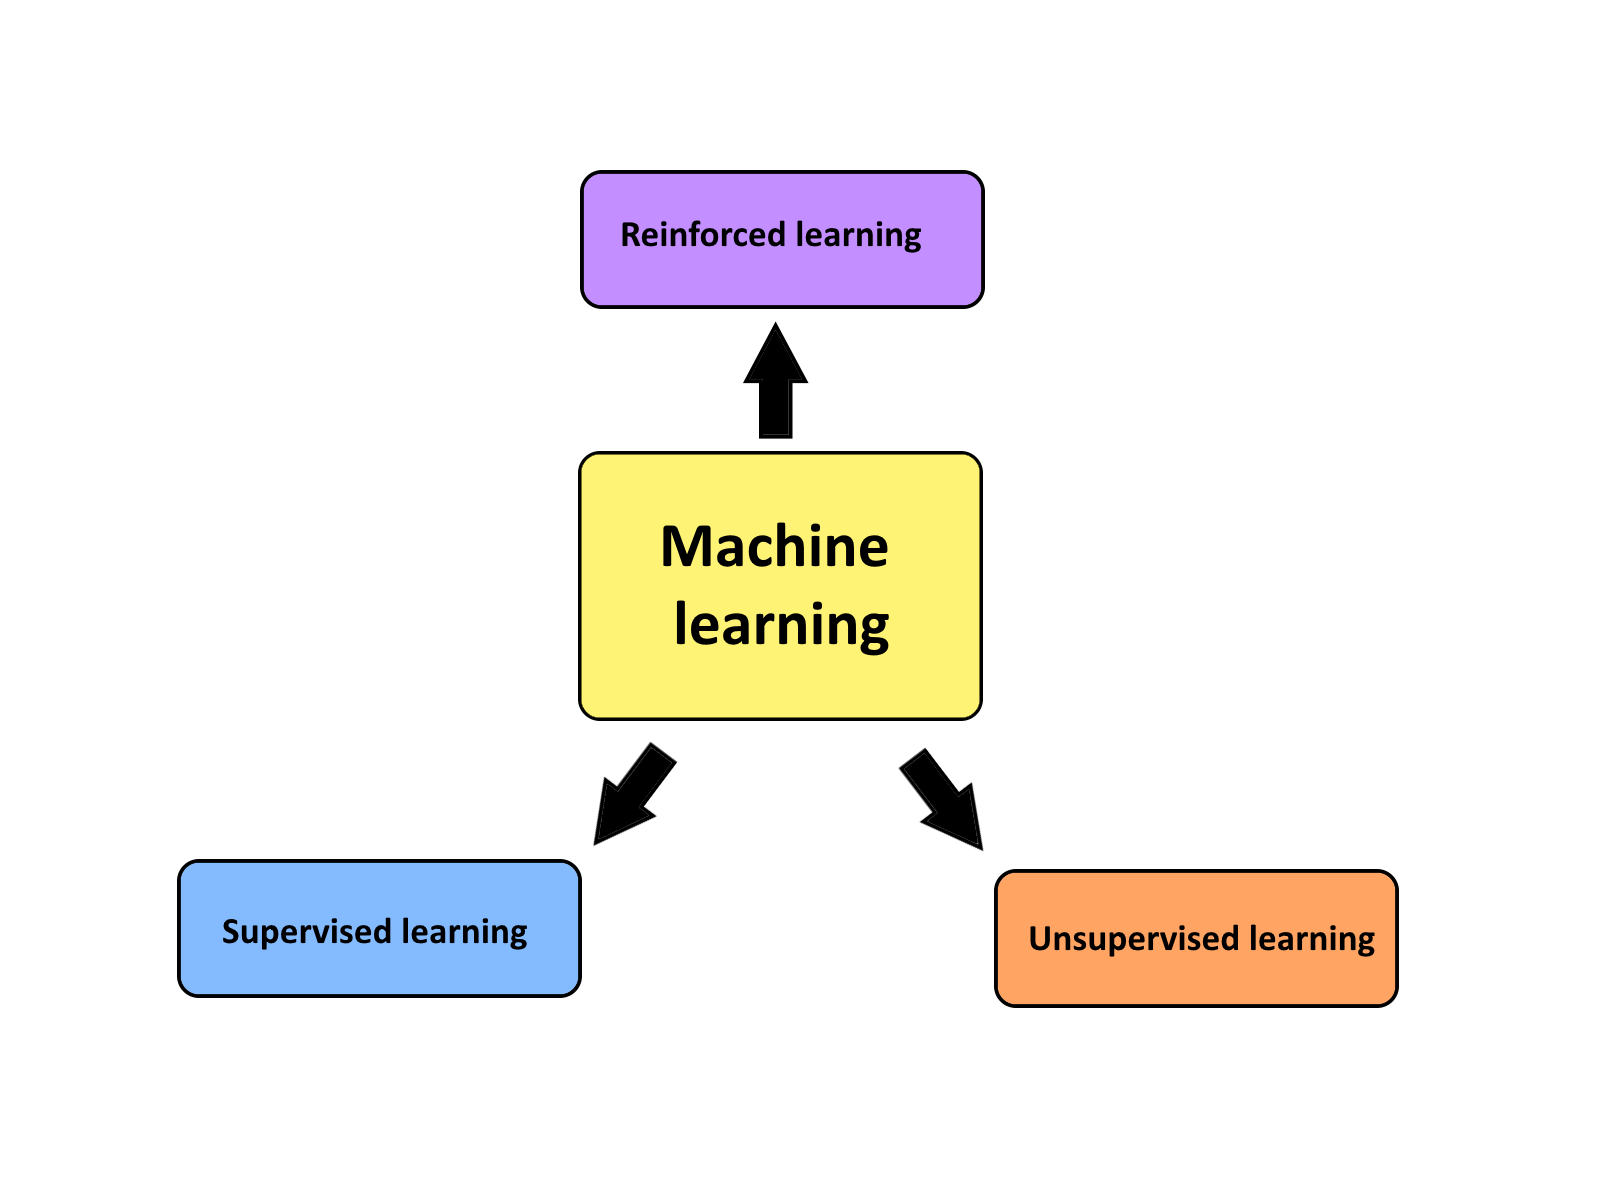
\includegraphics[width=\linewidth]{Overview_ml}
  \caption{Overview of the Machine Learning Strategy's.}
  \label{fig:overview_ML}
\end{figure}

Only the Supervised Learning strategy will be explained in more detail on the following pages, as the focus of this 
thesis lays in the comparision of several different implementations of classification algortihms that are based on 
Supervised Learning.
 

\cite{IntroML}

\subsection{Supervised Learning}

The idea behind Supervised learning is to create a model from a already labeled training data set, that then can make 
prediction and decision on new or unknown data based on the learned model from the training set. 
The following example will help to understand this easier.
Lets say a fruit farmer wants to automatically sort the harvested Fruits in either categorie A or B for the market. 
The sorting device is equiepped with 2 sensors to measure 2 features, one for colour and another one for the size of the 
fruit. It then decides to wich of the two classes the fruit belongs to. As this is a System that is capable of dividing 
features into a discrete number of classes the system can be called a \textit{classifier}. 
This is a typical exampel of an \textit{classifiecation task}.
To configure the System in such a way that it correctly sorts the fruits into the right category, 
a specailist hand picks several fruits from a small test set and then sorts them depending on the already named features. 
In other words, the specailist classiefies them. Based on this by hand sortet training set the machine will then later 
decide how the other fruits should be sorted. It is used as a \textit{model} for the classification. \cite{IntroAI}
Another type of Supervised learning is the \textit{regression task}. The difference to the \textit{classification task} is, 
that instead of a \textit{discrete} number of classes that gets returned, a \textit{continous} number of classes will be 
returned. An example of a \textit{regressive task} is, for example, the prediction of the Stock market or the price of 
medications.

The Process as seen in figure \ref{fig:sl_process} and as described as in the example of the farmer and his sorted 
fruits shows how the supervised learning works. The Algorithm (marked in green) learns with the help of the labeled 
training data. The result of this learning is then that the trained Algorithm, now called predictive model, 
can be used in a production enviroment.
New, unlabeled, data can then be send into the predictiv model to get a predictied model as an output. \cite{PythonML}

To better understand how this predictiv model is formed, one has to understand how the classification task works. 
In the classification task the computer programm is asked to specify which of \textit{k} catergories a input belongs to. 
To solve this task, the learning algorithm is usually asked to produce a function \textit{f} : $\R{}$ $\rightarrow$ ${1,...,k}$. 
When \textit{y} = \textit{f}(\textit{\textbf{x}}), the model assigns an input described by vector \textit{\textbf{x}} to a 
category identified by numeric code \textit{y}.
There are other variants of the classification task, for example, where \textit{f} outputs a probability distribution over 
classes. An example of a classification task is object recognition, where the input is an image (usually described as a set 
of pixel brightness values), and the output is a numeric code identifying the object in the image. \cite{Goodfellow-et-al-2016}

\pagebreak

\begin{figure}
  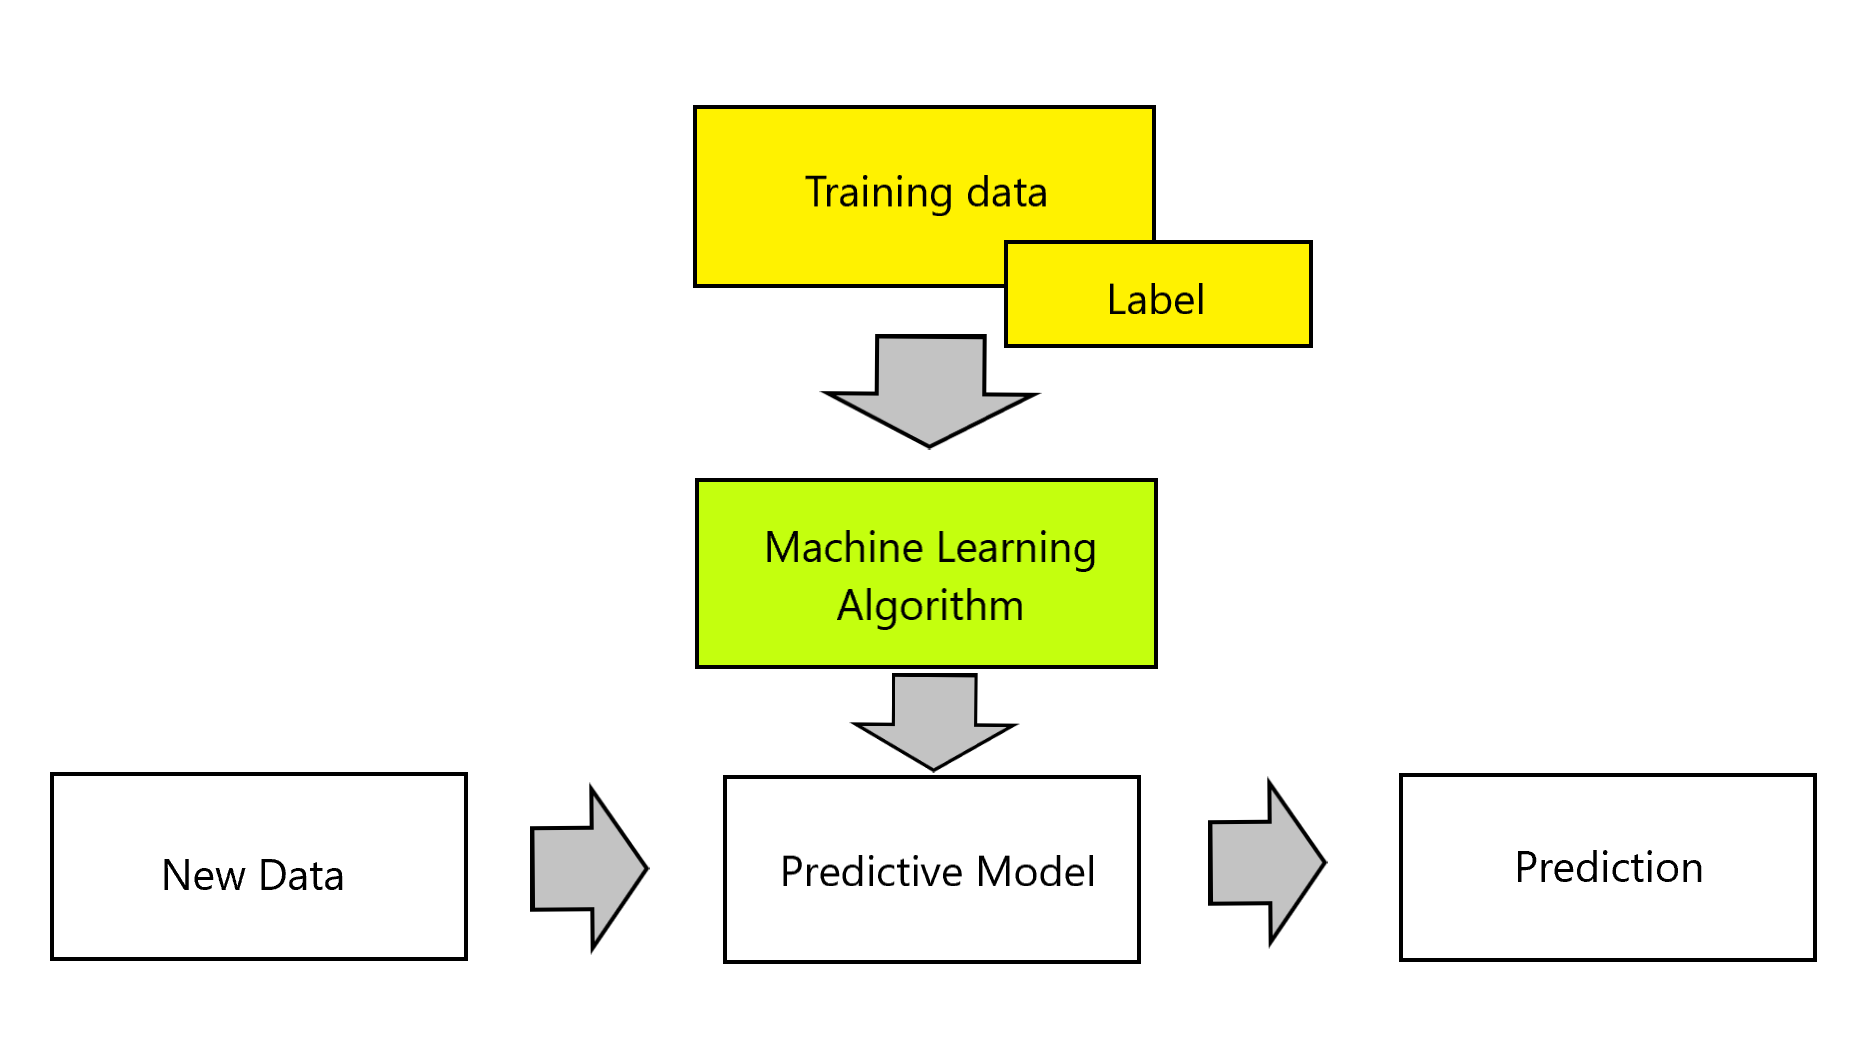
\includegraphics[width=\linewidth]{SL_process_figure}
  \caption{Process of the Supervised Learning. \cite{PythonML}}
  \label{fig:sl_process}
\end{figure}

Then there must be also differentiated between the type of data that is put into the classification process.
In batch or offine classification, a classifier-building algorithm is given a set of labeled examples. 
The algorithm creates a model, a classifier in this case. The model is then deployed, that is, used to predict the label 
for unlabeled instances that the classifier builder never saw. If we go into more detail, we know that it is good 
methodology in the first phase to split the dataset available into two parts, the training and the testing dataset, 
or to resort to cross-validation, to make sure that the classifier is reasonably accurate.
But in any case, there is a first training phase, clearly separated in time from the prediction phase.

In the online setting, and in particular in streaming, like it is this thesis, this separation between training, 
evaluating, and testing is far less clear-cut, and is interleaved. We need to start making predictions before we have all 
the data, because the data may never end. We need to use the data whose label we predict to keep training the model, 
if possible. And probably we need to continuously evaluate the model in some way to decide if the model needs more or 
less aggressive retraining. \cite{MLonDataStreams}

\pagebreak

\subsection{Gradient Descent}
The Gradient descent Algorithm is one of the most popular Algorithms to perform optimizations on and is by far the most 
commen way to optimize neural networks.This is also the reason why nearly every state-of-the-art Deep learning library 
has various forms of implementations to perform optimization on the gradient descent. The Problem, however is, that these
Algorithms often perform as some form of black-box, because a practical explanation of what their stengths and weaknesses 
is are hard to find and explain.
Gradient descent is a way to minimize an objective function \textit{J}($\theta$) parameterizedby a model's parameters $\theta \in \R{}^d$ by 
updating the parameters in the opposite directionof the gradient of the objective function $\nabla_\theta \in $\textit{J}($\theta$) with respect to 
the parameters. The learning rate $\eta$ determines the size of the steps wetake to reach a local minimum. In other words, 
we follow the direction of the slopeof the surface created by the objective function downhill until we reach a valley. \cite{overvieDiffRSLVQ}

The normal gradient descent, also known as batch-gradient descent, computes the gradient of the functionwith 
respect to the parameters $\theta$ for the entire training set:

\begin{equation}
\theta = \theta - \eta * \nabla_\theta \textit{J}(\theta)
\end{equation}

Since we need to calculate the gradients for the complete dataset to get just one update, batch gradient descent can get very
slow and is intractable for dataset that do not fit into the memory. For this reason the batch gradient descent implementation can not be used in this comparison,
as it is not able to perform updates "on-the-fly", as this is a necessarity for use on streaming Data. 

In contrast to that, the Stocastic Gradient Descent (short: SGD) can perform a update for \textit{each} training example
$\textit{x}^\textit{(i)}$ and label $\textit{y}^\textit{(i)}$:

\begin{equation}
\theta = \theta - \eta * \nabla_\theta \textit{J}(\theta;\textit{x}^\textit{(i)};\textit{y}^\textit{(i)})
\end{equation}

While the bacht gradient descent performed redudant computations for large datasets, as it recomputes gradients for similar examples 
before each update, the SGD puts away this redundacy by performing one update at a time. Because of that it performce much faster and 
can be used on Streaming Data.
The SGD performs frequent updates with a high variance, that causes the objective function to fluctuate heavily. 

\begin{figure}
  \centering
  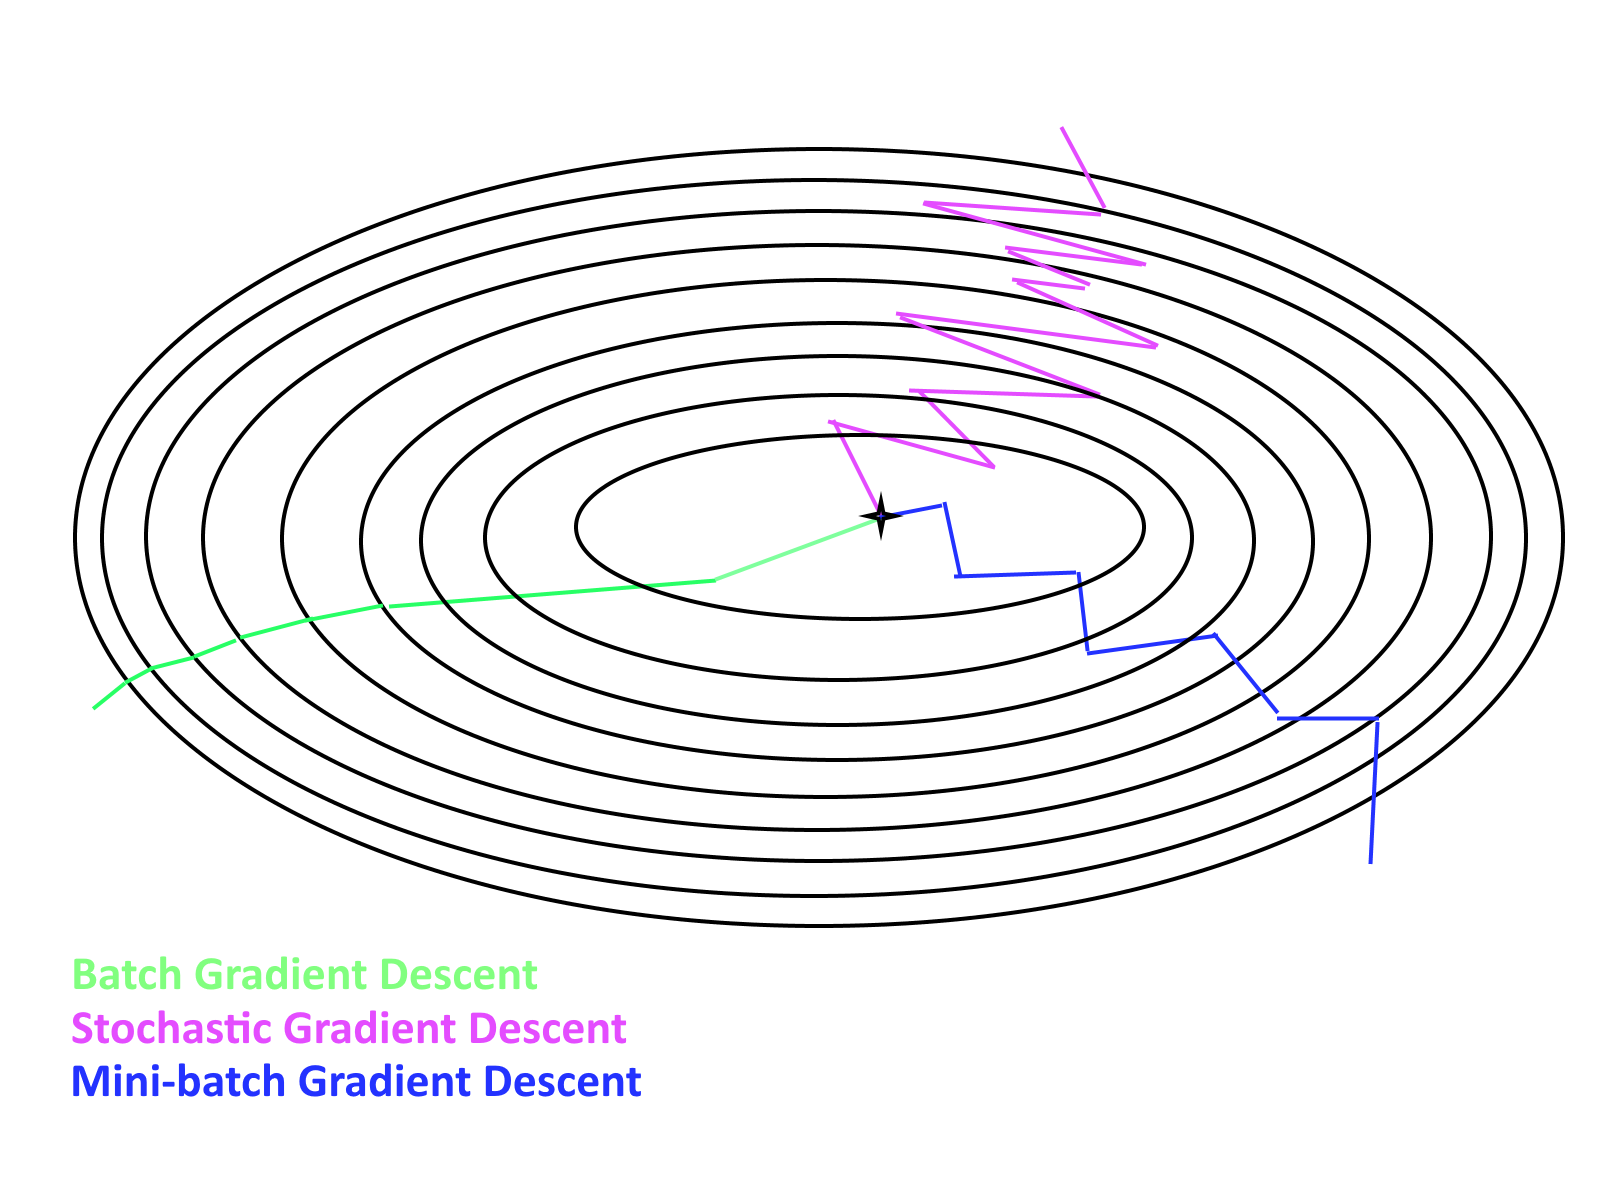
\includegraphics[width=0.7\columnwidth]{Gradient_desc_types}
  \caption{Visualisation differences of the three Gradient Descent Algorithms}
  \label{fig:comp_GD}
\end{figure}

This fluctuation enables the SGD to jump to new and potetially better local minima, while the batch gradient only converges 
to the minimum of the basin the parameters are placed in. But this also ultimatly complicates the convergensto the exact minimum, 
as the SGD keeps overshooting. This can be fixed by slowly decreasing the learning rate, as the SGD then shows the same 
convergeance behaviour as the batch gradient descent. It then almost certainly converges to a local or gloabl minimum for
non-convex and convex optimization respectivly. \cite{overvieDiffRSLVQ}
These advantages lead to the fact that the SGD is the most common Gradient descent algorithm.

Then there is also the Mini-batch gradient descent algorithm. It takes the best of both worlds and performs an update for
every mini-batch on \textit{n} training examples:

\begin{equation}
\theta = \theta - \eta * \nabla_\theta \textit{J}(\theta;\textit{x}^\textit{(i:i+n)};\textit{y}^\textit{(i:i+n)})
\end{equation}

This way it reduces the variance of the parameter updates, which can lead to a more stable convergence.
It can also make use of highly optimized matrix optimizations common for state-of-the-art deep learning libraries,
that makes computing the gradient with respect to a mini-batch very efficient. 
Common mini-batch sizes range between 50 and 256 , but can vary for different applications. Typically the Mini-batch gradient descent is the 
algorithm of choice when there is a neural network to train and the term SGD is usually also employed even when a mini-batches
are used. \cite{overvieDiffRSLVQ}

\pagebreak

\section{Streaming Data}

Data streams are an algorithmic abstraction to support real-time analytics. They are sequences of items, 
possibly infinite, each item having a timestamp, and so a temporal order. Data items arrive one by one, 
and we would like to build and maintain models, such as patterns or predictors, of these items in real time. 
There are two main algorithmic challenges when dealing with streaming data: the stream is large and fast, 
and we need to extract information in real time from it. That means that usually we need to accept approximate 
solutions in order to use less time and memory.
Also, the data may be evolving, so our models have to adapt when there are changes in the data. \cite{MLonDataStreams}

\subsection{Challenges with Streaming Data}

\cite{ConceptDrift}

\section{Framework}
The following section will shortly introduce the python based scikit-multiflow framework, with which the the comperssion 
of the different implementations of the RSLVQ algorithm where done.

\subsection{SCIKIT-Multiflow}
Scikit-multiflow is a framework that is inspired by the Massive Online Analysis (MOA), the most popular open source framework for machine learning on data streams,
and MEKA, an open source implementation of methods for multi labeling. Scikit-multiflow is also inpired by scikit-learn, the most 
popular framework for machine learning in Python. Following the Scikit philosophy, scikit-multiflow is an open source machine-
learning framework for multi-output/multi-label and stream data. 

The Scikit-multiflow does not provide a graphical user interface like the MOA framework that it was inspired by. 
On the other hand can it be used within Jupyter notebooks, a popular interface in the data scientist community that is based 
on python. 
It is mainly a library that contains stream generators, learning methods, change detectors and evaluation methods for 
Machien learning algorithms on streaming data. 
Scilit-multiflow lays a special focus on its design, so that it is user friendly to new user and familiar for more 
experienced ones.\cite{skmultiflow}

It achieves this by having a simple workflow that can be easily describe in 4 steps:

\begin{enumerate}
  \item Create a stream: \\
        A stream can be generate by use of either one of the predefiend Stream generators or by importing a Stream from a file.
  \item Instantiate a classifier: \\
        In this step the user has to choose by which type of algorithm the classifikation process should be accomplished.
  \item Setup the evaluator: \\
        Next the user has to choose if the evaluation process should be done presequential or by Hold-out method.
  Prequential-evaluation or interleaved-testthen-train evaluation, is a popular performance 
  evaluation method for the stream setting only, where tests are performed on new data before using it to train the model.
  Hold-out evaluation is a popular performance evaluation method for batch and stream settings, where tests are performed 
  in a separate test set. \cite{skmultiflow}
  \item Run the evaluation: \\
        The evaluator will perform the following subtask in this final step,
  first, it will check if there are still samples in the stream and then it will pass the next sample to the classifier,
  which will either test the sample with the \verb|predict()| method or it willl update the classefier with the \verb|partial_fit()|
  method of the clasifier.
\end{enumerate}
  
To give better understanding how this exactly works, \ref{lst:scikit} will provide a small example where a synthetic waveform gets 
generated with the WaveformGenerator. This generator will create a synthetic stream that generates default samples with
21 numeric attributes and 3 target values, based on a random differentiation of some base waveforms.
For the classifier is the Hoeffding Tree choosen with default parameters.
After this we chose a prequential evaluator with the following parameters: 
\begin{itemize}
  \item \verb|show_plot| = true, this will generate us a dynamic plot that will update as the classifier is trained.
  \item \verb|pretrain_size| = 200, this parameter sets the number of samples that is used for the first training set.
  \item \verb|max_sample| = 20000, this parameter set the maximum number of samples that should be used.
\end{itemize}
In the last step we then call evaluator method, that will then update the results and the plot.
It is to note that at the time this thesis was written, the accuracy score stand for the performance 
in the framework.  \cite{skmultiflow}

\begin{lstlisting}[label=lst:scikit,
  language=python,
  firstnumber=1,
  caption=Simple example of the scikit-multiflow workflow]			   

  """1. Create a stream""" 
  stream = WaveformGenerator()
  stream.prepare_for_use()
  
  """2. Instantiate the HoeffdingTree classifier"""
  ht = HoeffdingTree()
  
  """3. Setup the evaluator"""
  evaluator = EvaluatePrequential(show_plot=True,
                                  pretrain_size=200,
                                  max_samples=20000)
  
  """4. Run evaluation"""
  evaluator.evaluate(stream=stream, model=ht)
\end{lstlisting}

\begin{figure}[H]
  \centering
  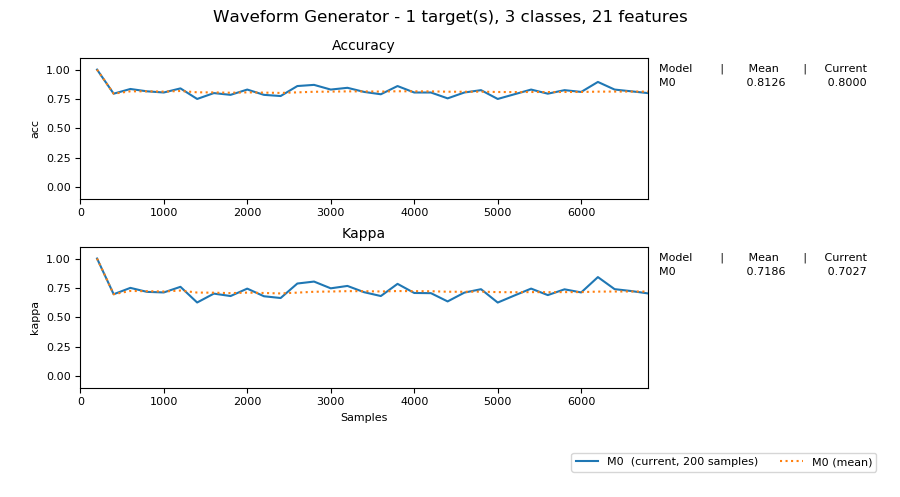
\includegraphics[width=\columnwidth]{Scikit_multiflow_example}
  \caption{Result Table of the example in \ref{lst:scikit}} 
  \label{fig:sci_result_examp}
\end{figure}

\section{Criteria for the Comparision}

This section will explain on what criteriy this thesis will base the comparsion of the different implementations. 
It will also descirbe what the difference between the cireria is and why this is importend to know.
It will define what this thesis understands under the terms performance and accuracy, as well as what the differences
between the used error-estimations are.

\subsection{Evaluations for Data Streams}
To evaluate a learning algorithmus, it must be know which examples were used to train the algorithmus and which are used to 
test the model output by the algorithms. Which procedure is used in batch learning has partly depended on data size.
For small data sets with < 1000 examples the procedure of cross-validation was well suited, as it made maximum use of the
data that it could use.
A Problem arose when the size of the data keept increasing, as this practicly created a time limit for procedures that keept
repeating the training process to many times.
For this reason it is commen practise to try to reduce the number of folds and repetitions for big data sets to allow experiments
to conclude in reasonable time. 
One way to achieve this is to take several hundreds of thousend samples in a single batch and take them for a single holdout run,
as this requires the least computational effort. The rationalization for this, beside the practical time issues, is that the 
reliability we may lose by not having repeated runs is compensated by the reliability gained by the sheer number of samples that are used. 
There are two main approaches that we have to consider for the evaluation process, the first one being Holdout and the second being 
Prequential. \cite{Bifet_datastream} \\
These two approaches will be now be described in more detail:

\begin{itemize}
  \item \textbf{Holdout}:
        It is often acceptable to measure the performance with a single holdout set when the batch learning learning 
        would otherwise reache a scale where cross-validation would be too time consuming.
        This can get very helpful, as the results of different studies can be directly compared to each other. 
        To do this, the division between the train and test set have to be predefiened.
        To track model performance over time, the model can be evaluated periodically, for example, after every 
        one million training examples. Testing the model too often has potential to significantly slow the evaluation 
        process, depending on the size of the test set.
        A source for holdout dat sets are for example sets of data of the stream that have not yet been used to train 
        the learning algorithm.
        These sets could be taken from "further ahead" in the stream to be used as test sets and could then later be 
        used again to train the learning algortihm again after the testing is complete.
        This procedure would be recommandable in scenarios with concept-drift, as it would measure a model’s ability
        to adapt to the latest trends in the data.
        In scenarios without drift, a single static holdout set should be sufficent, as this would avoid varying estimates 
        between test sets.
        If it is assumed that the test set is independent and sufficently large in relation to the complexity of the 
        target concept, it can be concluded that it then will provide an accurate measurement of generalization accuracy.
        \cite{Bifet_datastream}
  \item \textbf{Prequential}:
        An alternative approach to evaluate data stream algorithm is to interleave testing with training. Each individual
        set can be used to test the model before it is used for training and then the accuracy can be incremantally updated
        from this. When it is performed in this order the model will always be tested by sets that it has not seen yet.
        This has the advantage that no holdout set is needed to perform testing. This also results in a smooth plot of 
        the accuracy over time, as each individual set will become increasingly more insignificant to the overall average.
        This approach also has its disadvantages, as it make it diffcult to accuratly seperate and measure
        training and testing times. It also obscures the true accuracy that the algorithm can achieve at agiven point, as the 
        algorithm gets punished for mistakes that it made earlier regardless of the level of accuracy they are eventually
        capable of. It also has to be said that this effect will diminish over time.
        With this approach the statistcs are updated with every set from the stream and can be recorded at this level od detail
        if desired. To increase the efficiency a sampling parameter can be used to reduce the required storage for the results,
        by recording only at periodic intervals like the holdout method.
        \cite{Bifet_datastream}
\end{itemize}

\subsection{Performance}
Performance is the ability of the classifier not to label as positive an instance that is negative.

\subsection{Accuracy score}
Accuracy is the number of instances correct clasified / total number of instances.

\chapter{Used Algorithms}

\section{Theoretical Work}

This chapter will try to give a short explanation about how the Robust Soft Learning Vector Quantization Algorithm 
(short: RSLVQ) works and will also explain the algorithm that it is based on. 
Furthermore will it explain what momentum based gradient descent algortihms there are and how they work.
These are used in the different optimization implementation of the RSLVQ that will be compared in the later chapters. 

\section{Learning Vector Quantization}

\section{Robust Soft Learning Vector Quantization}
The LVQ algorithm may be a popular adaptive nearest prototype classifier for multiclass classification, 
but the algortihms from this familiy had only been propsed on heuristic grounds. Seo and Obermayer then derived the 
Robust Soft Learning Vector Quantization (RSLVQ varient) in their work \cite{RSLVQOrig}. It is a LVQ that is based on 
a Gausian Mixture ansatz. It proposes an objective function which is based on a likelihood ratio and derives the
learning rule from gradient descent.

They asume that the following objective function is maximized:

\begin{equation}
  \begin{split}
    L_r &= \displaystyle\prod_{k=1}^{N} \frac{p(x_k, y_k\mid\tau)}{p(x_k, y_k\mid\tau) + p(x_k, \bar{y}_k\mid\tau)} \\
        &= \displaystyle\prod_{k=1}^{N} \frac{p(x_k, y_k\mid\tau)}{p(x_k\mid\tau)}  \overset{!}{=} max.
  \end{split}
\end{equation}

The ratio $\frac{p(x, y\mid\tau)}{p(x\mid\tau)}$ is bounded by 0 from below and bounded by 1 from above. Because of this, 
instead of optimizing the likelihood ratio, they then optimize the 
logarithm of the ratio $L_r$ like this,

\begin{equation}
    log L_r = \displaystyle\sum_{k=1}^{N}log\frac{p(x_k, y_k\mid\tau)}{p(x_k\mid\tau)} \overset{!}{=} max,
\end{equation}

were Stochastic gradient descent leads to the following learning rule:

\begin{equation}
  \theta_l(t + 1) = \theta_l(t) + \alpha(t)\frac{\partial}{\partial\theta_l} [log \frac{p(x, y\mid\tau)}{p(x\mid\tau)}]
  \label{equ:RSLVQ_1},
\end{equation}

where $\alpha(t)$ is learning rate with $\sum_{t=1}^{\infty} \alpha(t) = \infty$ and $\sum_{t=1}^{\infty} \alpha^2(t) < \infty$.
If the conditional density functions $p(x\mid j)$ are of the normalized exponential form

\begin{equation}
  p(x\mid j) = K(j) exp f(x, \theta_j), 
\end{equation}

the learning rule becomes

\begin{equation}
  \begin{split}
    &\frac{\partial}{\partial\theta_l} [log \frac{p(x, y\mid\tau)}{p(x\mid\tau)} = \delta(c_l = y)(P_y(l\mid x) - P(l\mid x))\frac{\partial f(x, \theta_l) }{\partial\theta_l} \\
    &- \delta(c_l \neq y) P(l\mid x)\frac{\partial f(x, \theta_l) }{\partial\theta_l}.
  \end{split}
\end{equation}

where $P_y(l\mid x)$ and $P(l\mid x)$ are assigment probabilities,

\begin{equation}
  \begin{split}
    P_y(l\mid x) &= \frac{p(l) exp f(x, \theta_l)}{\displaystyle\sum_{j:c_j = y}p(j) exp f(x, \theta_j)}, \\
    P(l\mid x) &= \frac{p(l) exp f(x, \theta_l)}{\displaystyle\sum_{j=1}^{M}p(j) exp f(x, \theta_j)}.
  \end{split}
\end{equation}

$P_y(l\mid x)$ describes the (posterior) probability that the data point \textit{x} is assigned to the component \textit{l} of the mixture
, given that the data point was generated by teh correct class. $P(l\mid x)$ describes teh (posterior) probability that the 
data point \textit{x} is assigned to the component \textit{l} of the complete mixture using all classes.
Using the gradient given by the equation \ref{equ:RSLVQ_1}, following learning rule is obtained: 

\begin{equation}
  \theta_l(t + 1) = \theta_l(t) + \alpha(t) 
  \begin{cases}
    P_y(l\mid x) - P(l\mid x)[\frac{\partial f(x, \theta_l) }{\partial\theta_l}], c_l = y,  \\
    - P(l\mid x)[\frac{\partial f(x, \theta_l) }{\partial\theta_l}],              c_l \neq y.              
  \end{cases}
  \label{equ:RSLVQ_2}
\end{equation}

It has to be noted that the factor $P_y(l\mid x) - P(l\mid x)$ is always positive. \cite{RSLVQOrig}

The Cost-function and the learning rule described until now were for training the RSLVQ for the general case, but 
Seo and Obermayer provided also a varient that uses a Gaussian mixture ansatz.
In that version they choose a Gaussian mixture model whose components have similar width and strengths, i.e.
$\sigma_l = \sigma, \forall l, and$ $p(l) = \frac{1}{M}, l = 1, ..., M$. They obtain 

\begin{equation}
  f(x,\theta_l) = \frac{-(x-\theta_l)^2}{2\sigma^2},   \quad   \frac{}{}f(x,\theta_l) = \frac{1}{\sigma^2}(x-\theta_l).
\end{equation}

By substituting the derivative of $f(x,\theta_l)$ into equation \ref{equ:RSLVQ_2} they obtained

\begin{equation}
  \theta_l(t + 1) = \theta_l(t) + \alpha(t) 
  \begin{cases}
    P_y(l\mid x) - P(l\mid x)(x-\theta_l), \quad c_l &= y,  \\
    - P(l\mid x)(x-\theta_l),               c_l &\neq y,              
  \end{cases}
  \label{equ:RSLVQ_3}
\end{equation}

where $\alpha(t) = \frac{\alpha(t)}{\sigma^2}$ and

\begin{equation}
  \begin{split}
    P_y(l\mid x) &= \frac{exp \frac{-(x-\theta_l)^2}{2\sigma^2}}{\displaystyle\sum_{j:c_j = y} exp \frac{-(x-\theta_j)^2}{2\sigma^2}}, \\
    P(l\mid x) &= \frac{exp \frac{-(x-\theta_l)^2}{2\sigma^2}}{\displaystyle\sum_{j=1}^{M} exp \frac{-(x-\theta_j)^2}{2\sigma^2}}.
  \end{split}
  \label{equ:RSLVQ_4}
\end{equation}

The equations \ref{equ:RSLVQ_3} and \ref{equ:RSLVQ_4} implement the RSLVQ algorithm. Prototypes whose label is equal to 
the label of the data point are attracted, while prototypes with different labels are repelled. Using deterministic annealing
of $\sigma^2$, which is a hyperparameter of the learning rule described in \ref{equ:RSLVQ_3}, the RSLVQ can be optimized.
If the width $\sigma$ of the Gaussian components goes to zero, both assignment probabilities (equation \ref{equ:RSLVQ_4}),
become hard assignments. If th label $c_q$ of the nearest prototype \textit{q} is equal to the label \textit{y} of the data
point \textit{x} then no update is being performed, because 

\begin{equation}
  P(l\mid x) = P_y(l\mid x) = 0, \quad \forall l \neq q, \quad P_y(q\mid x)-P(q\mid x) = 0.
\end{equation}

Only if the label of the data point \textit{x} differs from the label of the nearest prototype \textit{q}, then

\begin{equation}
  \begin{split}
    P(l\mid x) &= 0, \forall l \neq q, \quad \quad P_y(l\mid x) = 0, \forall l \neq q',\\
    P(q\mid x) &= 1, \quad \quad \quad \quad \quad P_y(q\mid x) = 1,
  \end{split}
\end{equation}

where \textit{q'} is the nearest prototype vector with the correct class label, and the nearest prototype vector and the 
nearest correct prototypevector are changed. In the "hard" version of the RSLVQ, prototypes are modified only by the data 
points that are not correctly classified. \cite{RSLVQOrig}

Seo and Obermayer then showed in their work \cite{RSLVQOrig} for LVQ 2.1 data points which are near the current 
class boundary and which are classified correctly have the strongest effect on the update of the prototypes. In contrast to that
relies the RSLVQ on data points which are further away from the classification boundary and which are incorrectly classified,
i.e. RSLVQ learns from mistakes. Additionaly, the RSLVQ does not require a "window rule" like the LVQ 2.1, as the prototypes 
do not diverge. \cite{RSLVQOrig}

\section{Momentum Based Gradient Descent}

The following section will outline three algorithms that are widely used in the Deep learning Community and that will later
be used to optimize the RSLVQ Algorithm in hopes to improve its performence and accuracy.

\subsection{Momentum}

SGD has trouble navigating ravines, i.e. areas where the surface curves much more steeply in one dimension than in another \cite{problemSteepLearn, overvieDiffRSLVQ},
which are common around local optima. In these scenarios, SGD oscillates across the slopes of the ravine while only making 
hesitant progress along the bottom towards the local optimum as in figure.

\begin{figure}[H]
  \centering
  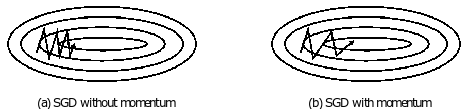
\includegraphics[width=\columnwidth]{SGD_momentum}
  \caption[Diff. SGD moment.]{Differences of a SGD with and without momentum.\footnotemark} 
  \label{fig:SGD_momentum}
\end{figure}

Momentum \cite{QIAN1999145, overvieDiffRSLVQ} is a method that helps accelerate SGD in the relevant direction and dampens
oscillations as can be seen in figure . It does this by adding a fraction $\gamma $ of the update vector of the past time step to the
current update vector

\begin{equation}
\begin{split}
\textit{v}_\textit{t} &= \gamma\textit{v}_\textit{t-1} + \eta \theta - \eta\nabla_\theta \textit{J}(\theta) \\
\theta &= \theta - \textit{v}_\textit{t}
\end{split}
\end{equation}

The momentum term $\gamma $ is usualy set to 0.9 or a similar value.

In his Article, Ruder \cite{overvieDiffRSLVQ} describs it like if we would push a ball down a hill. 
The ball accumulates momentum as long as it rolls downhill, becoming faster and faster on the way 
(until it reaches its terminal velocity, if there is air resistance, i.e. $\gamma $ < 1). 
The same thing happens to our parameter updates: The momentum term increases for dimensions whose gradients
point in the same directions and reduces updates for dimensions whose gradients change directions.
As a result, we gain faster convergence and reduced oscillation.
\footnotetext{Genevieve B. Orr}

\subsection{Adagrad}
The first algorithm that will be described is the Adagrad \cite{Zeiler2012ADADELTAAA}. It has to be noted that this 
algorithm will not be part of the comparision, but as this algorithm is the base from wich the Adadelta and later the 
RMSprop were developed from, it will be shortly explained nonteless.
The Adagrad is an algorithm for gradient-based optimization that adapts to updates for each individual parameter to 
perform larger or smaller updates depending on their importance. The learning rate gets adapted to the parameters, were
it performs larger updates if the parameters are more infrequent and smaller updates if they are frequent.
Hence, it is well-suited to deal with sparse data. As other works \cite{dean2012large} have shown, this greatly improves
the robustness of SGD, which lead to its wide use to train large Neural Networks.
It was also used to train GloVe word embeddings as infrequent words require
much larger updates than frequent ones \cite{pennington2014glove, overvieDiffRSLVQ}.   

For the reason that Adagrad uses a different learning rate for every parameter $\theta_i$ at every time step \textit{t},
Adagrad's per-parameter update is first shown and then vectorized. For brevity, we set $\textit{g}_\textit{t, i}$ to be
the gradient of the objective function w.r.t. the parameter $\theta_i$ at the time step \textit{t}:

\begin{equation}
  \textit{g}_\textit{t, i} = \nabla_\textit{$\theta$ t}\textit{J}(\theta_\textit{t, i})
  \label{equ:Adagrad_1}
\end{equation}

The update for every SGD parameter $\theta_i$ at time \textit{t} becomes to:

\begin{equation}
  \theta_\textit{t+1, i} = \theta_\textit{t, i} - \eta \cdot \textit{g}_\textit{t, i}
\end{equation}

In its update rule, Adagrad modifies the general learning rate $\eta$ each time step \textit{t} for every parameter
$\theta_i$ based on the past gradients that have been computed for $\theta_i$:

\begin{equation}
  \theta_\textit{t+1, i} = \theta_\textit{t, i}-\frac{\eta}{\textit{G}_\textit{t, ii} - \epsilon} \textit{g}_\textit{t, i}
\end{equation}

$\textit{G}_t$ $\in$ $\R^\textit{dxd}$ here is a diagonal matrix where each diagonal element \textit{i, i} is the sum of the
squares of the gradients w.r.t. $\theta_i$ up to time step \textit{t} \cite{AdadeltaAddition}, while $\epsilon$ is a smoothing term that avoids
division by zero (usually on the order of 1\textit{e} - 8). 

As $\textit{G}_t$ contains the sum of the squares of the past gradients w.r.t. to all parameters $\theta$ along its
diagonal, we can now vectorize our implementation by performing an element-wise matrix-vector multiplication $\odot$
between $\textit{G}_t$ and $\textit{g}_t$:

\begin{equation}
  \Delta\theta_\textit{t} = -\frac{\eta}{\sqrt{\textit{G}_\textit{t} + \epsilon}} \odot \textit{g}_\textit{t}
  \label{equ:Adagrad_2}
\end{equation}

One of Adagrad’s main benefits is that it eliminates the need to manually tune the learning rate. Most implementations 
use a default value of 0.01 and leave it at that.
Adagrad’s main weakness is its accumulation of the squared gradients in the denominator: Since every added term is 
positive, the accumulated sum keeps growing during training. This in turn causes the learning rate to shrink and eventually
become infinitesimally small, at which point the algorithm is no longer able to acquire additional knowledge. \cite{overvieDiffRSLVQ}

\subsection{Adadelta}
One of the more often used momentum-based algorithm is the Adadelta approach. It is an extension of the Adagrad that 
seeks to reduce its aggressive, monotonically decreasing learning rate. Instead of accumulating all past squared gradients, 
Adadelta restricts the window of accumulated past gradients to some fixed size $\omega$.  

Rather than inefficently storeing $\omega$ previous squared gradients, the sum of gradients is recursively defined as a 
decaying average of all past squared gradients. The running average $\textit{E}[\textit{g}^2]_t$  at time step \textit{t} 
then depends (as a fraction $\gamma $ similarly to the Momentum term) only on the previous average and the 
current gradient:

\begin{equation}
\textit{E}[\textit{g}^2]_t = \gamma\textit{E}[\textit{g}^2]_\textit{t-1} + (1-\gamma)\textit{g}^2_t
\end{equation}

We then set $\gamma$ to a simliar value as the momentum, around 0.9. The SGD update will then be rewriten in terms of the 
parameter update vector $\Delta\theta_\textit{t}$:

\begin{equation}
  \begin{split}
    \Delta\theta_\textit{t} &= -\eta \cdot \textit{g}_\textit{t,i} \\
    \theta_\textit{t+1} &= \theta_\textit{t} - \Delta\theta_\textit{t}
  \end{split}
\end{equation}

Because of this, the parameter update vector, that is base of the parameter update vecotor of the Adagrad (see equation \ref{equ:Adagrad_2}), 
takes the form of:

\begin{equation}
  \Delta\theta_\textit{t} = -\frac{\eta}{\sqrt{\textit{G}_\textit{t} + \epsilon}} \odot \textit{g}_\textit{t}
\end{equation}

In the next step the diagnoal Matrix $\textit{G}_t$ gets replaced with the decaying average over past squared gradients 
$\textit{E}[\textit{g}^2]_\textit{t}$:

\begin{equation}
  \Delta\theta_\textit{t} = -\frac{\eta}{\sqrt{\textit{E}[\textit{g}^2]_\textit{t} + \epsilon}} \textit{g}_\textit{t}
\end{equation}

As the denominator is just the root mean squared (RMS) error criterion of the gradient, we can replace
it with the criterion short-hand: 

\begin{equation}
  \Delta\theta_\textit{t} = -\frac{\eta}{RMS[\textit{g}]_t} \textit{g}_\textit{t}
\end{equation}

As in \cite{AdadeltaAddition} noted, the units in this update (as well as in the SGD, Momentum and Adagrad) do not match,
i.e. the update should have the same hypothetical units as the parameter. To realize this, they first define another 
ecaying average, this time not of squared gradients but of squared parameter updates:

\begin{equation}
  \textit{E}[\Delta\theta^2]_t = \gamma\textit{E}[\Delta\theta^2]_t-1 + (1-\gamma)\Delta\theta^2_t
\end{equation}

This leads to that the root mean squared error of the parameter updates is:

\begin{equation}
  \textit{RMS}[\Delta\theta]_t = \sqrt{\textit{E}[\Delta\theta^2]_t + \epsilon}
\end{equation}

Because the $\textit{RMS}[\Delta\theta]_t$ value is unknown to us, we try to approximate it with the \textit{RMS} of 
parameter updates until the previous time step. Replacing the learning rate $\eta$ in the previous update rule with $\textit{RMS}[\nabla\theta]_t-1$
leads to the final update rule for the Adadelta:

\begin{equation}
  \begin{split}
  \Delta\theta_t &= - \frac{\textit{RMS}[\Delta\theta]_\textit{t-1}}{RMS[\textit{g}]_t} \textit{g}_\textit{t} \\
  \theta_\textit{t+1} &= \theta_t + \Delta\theta_t
  \end{split}
\end{equation}

In the Adadelta we do not need to set a learning rate $\eta$, eliminated from the update rule. \cite{overvieDiffRSLVQ}

\subsection{RMSprop}
RMSprop is an adaptive learning rate method proposed by Geoff Hinton in Lecture 6e of his Coursera Class. \cite{RMSprop_Hinton}
As a result of the need to resolve the Adagrad's radically diminishing learning rates, both the Adadelta and 
the RMSprop had been developed independetly from each other at the same time. RMSprop in fact is identical
to the first update vector of Adadelta that we derived above:

\begin{equation}
  \begin{split}
  \textit{E}[\textit{g}^2]_t &= 0.9\textit{E}[\textit{g}^2]_\textit{t-1} + 0.1\textit{g}^2_t \\
  \theta_\textit{t+1} &= \theta_\textit{t}-\frac{\eta}{RMS[\textit{g}]_t} \textit{g}_\textit{t}
  \end{split}
\end{equation}

RMSprop as well divides the learning rate by an exponentially decaying average of squared gradients.
Hinton suggests $\gamma$ to be set to 0.9, while a good default value for the learning rate $\eta$ is 0.001. \cite{overvieDiffRSLVQ}

\subsection{Adam}
As described in \cite{Kingma2014AdamAM}, the Adaptive Moment Estimation (Adam) is another way to compute the adaptive 
learning rate for each parameter. Additionly to storing an exponentially decaying average of past squared gradients
$\textit{v}_t$ like Adadelta or RMSprop, Adam also keeps an exponentially decaying average of past gradients $\textit{m}_t$,
simliar to momentum:

\begin{equation}
  \begin{split}
  \textit{m}_t &= \beta_1\textit{m}_\textit{t-1} + (1-\beta_1)\textit{g}_t \\
  \textit{v}_t &= \beta_2\textit{v}_\textit{t-1} + (1-\beta_2)\textit{g}^2_t
  \end{split}
\end{equation}

$\textit{m}_t$ and $\textit{v}_t$ are estimates of the first moment (the mean) and the second moment (the uncentered variance)
of the gradients respectively, hence the name of the method. As $\textit{m}_t$ and $\textit{v}_t$ are initialized as vectors of 
0's, the authors of Adam observe that they are biased towards zero, especially during the initial time steps, and especially 
when the decay rates are small (i.e. $\beta_1$ and $\beta_2$ are close to 1).

To counteract these biases they compute a bias-corrected estimate of the first and second moment:

\begin{equation}
  \begin{split}
  \hat{m}_t &= \frac{\textit{m}_t}{1-\beta^t_1} \\
  \hat{v}_t &= \frac{\textit{v}_t}{1-\beta^t_2}
  \end{split}
\end{equation}

These are then used to update the parameters just as we have seen in Adadelta and RMSprop, which yields the Adam update rule:

\begin{equation}
\theta_\textit{t+1} = \theta_\textit{t}-\frac{\eta}{\sqrt{\hat{v}_t}+ \epsilon} \hat{m}_t
\end{equation}

The authors recommend in their work to use as default values of 0.9 for $\beta_1$, 0.999 for $\beta_2$ and $10^-8$ for $\epsilon$.
They show empirically that Adam works well in practice and compares favorably to other adaptive learning-method algorithms.
\cite{overvieDiffRSLVQ, Kingma2014AdamAM}

\begin{algorithm}
  \caption{Adam algorithm, as proposed in \cite{Kingma2014AdamAM}. The authors recommend for default settings the value
          0.9 for $\beta_1$, 0.999 for $\beta_2$ and $10^-8$ for $\epsilon$ as well as a stepsize $\alpha$ of 0.001.}\label{euclid}
  \begin{algorithmic}[1]
    \Require $\alpha$: Stepsize
    \Require $\beta_1$, $\beta_2$ $\in$ $[0,1)$: Exponential decay rates for the moment estimates
    \Require \textit{f}$(\theta)$: Stochastic objective function with parameters $\theta$
    \Require $\theta_0$: Initial parameter vector \\
    Initialize first moment vector: $m_0 = 0$ \\
    Initialize second moment vector: $v_0 = 0$ \\
    Initialize timestep: $t = 0$ 
    \While{$\theta_t$ not converged} \\
      t = t + 1 \\
      Get the gradients at timestamp $\textit{t}: \textit{g}_t \leftarrow \nabla_\textit{$\theta$ t}\textit{J}(\theta_\textit{t-1})$ ( see equation \ref{equ:Adagrad_1}) \\
      Update first moment estimate: $\textit{m}_t \leftarrow \beta_1\textit{m}_\textit{t-1} + (1-\beta_1)\textit{g}_t$ \\
      Update second moment estimate: $\textit{v}_t \leftarrow \beta_2\textit{v}_\textit{t-1} + (1-\beta_2)\textit{g}^2_t$ \\
      Compute bias-corrected first moment estimate: $\hat{m}_t \leftarrow \frac{\textit{m}_t}{1-\beta^t_1}$ \\
      Compute bias-corrected second moment estimate: $\hat{v}_t \leftarrow \frac{\textit{v}_t}{1-\beta^t_2}$ \\
      Update the parameters: $\theta_\textit{t+1} \leftarrow \theta_\textit{t}-\frac{\eta}{\sqrt{\hat{v}_t}+ \epsilon} \hat{m}_t$ \\
    \EndWhile
    \Return Resulting parameters: $\theta_t$
  \end{algorithmic}
\end{algorithm}

\section{Implementation of the RSLVQ variants}

\subsection{RSLVQ SGD}

\subsection{RSLVQ prop}

\subsection{RSLVQ adadelta}

\subsection{RSLVQ adam}

\chapter{Test realisation}

\section{Used Streaming Datat sets}

In this section will be a short describtion of the data streams, synthetic and real world data, that where used to 
perform the experiments.

\subsection{Synthetic data}

\begin{itemize}
  \item Sea Concepts: !not finsihed rework required!\\
        This dataset consists of 50000 instances with three attributes of which only two are relevant. 
        The two class decision boundary is given by f1 + f2 = b, where f1, f2 are the two relevant features and b a
        predefined threshold. Abrupt drift is simulated with four different concepts, by changing the value of b every 
        12500 samples. Also included are 10\verb|%| of noise. \cite{SEADataset}
  \item Moving Squares: \\
        placeholder
\end{itemize}

\subsection{Real world data}

\begin{itemize}
  \item Weather Dataset: \\
        This dataset contains eight different features like the minimum and maximum tempreature, visibility, wind speed, 
        air pressure, etc. that were measured at the Offutt Air Force Base in Bellevue, Nebraska. These measuredments were
        measured in the period of 1949-1999. The goal of this dataset is to predict if it is going to rain on certains day or not.
        It contains 18159 instances with an imbalance towards no rain (69\verb|%|) and was introduced by Elwell et al..

  \item Electicity Market Dataset:\\
        First described by Harris et al., it is often used for performance comparison, as it is a good benchmark for concept drift 
        classification. It holds the information of the Australian New South Wales Electricity Market, whose prices are affected 
        by supply and demand. Each sample is characterized by teh following attributes: day of the week, time stamp, market demand,
        etc.. Each of the samples refers to a period of 30 minutes and the class label identifies the relative change compared to the
        last 24 hours. The used Dataset is the normalized version of the original dataset.

  \item Poker Dataset: \\
        To create this dataset, one million poker hands, each represented by five cards that got encoded with its suit and rank, 
        were randomly drawn. The class is the resulting poker hand itself such as one pair, full house and so forth.
        Since the poker hand can not change by definition and each instance was randomly generated, this dataset had 
        in its original form no drift in it.
        As this is the version as it was introduced by \cite{bifet2013efficient}, virtual drift is present in this dataset. 
        This was achieved by sorting the instances of the dataset by rank and suit. Duplicate hands were also removed.
        Additionly, this version was also normalized.

  \item Outdoor Objects: \\
        This Dataset was optained by images that were recorded by a mobile in a garden enviroment. The goal is to classify 40 different objects,
        each approached ten times under varying lighting conditions affecting the color based representation.
        Every ten images represent one approach and each approach is in temporal order within the dataset.
        The objects are encoded in a normalized 21-dimensional RG-Chromaticity histogram.

\end{itemize}

\section{Implementation of the Comparision and Results}

\subsection{Experiment begrenzung}

\subsection{Experiment aufbau}

\subsection{Experiment durchlauf}

\begin{lstlisting}[label=lst:java,
				   language=java,
				   firstnumber=1,
				   caption=Beispiel für einen Quelltext]				   

public void foo() {				   
	// Kommentar
}
\end{lstlisting}

Lorem ipsum dolor sit amet, consectetur adipiscing elit. Ut vehicula felis lectus, nec aliquet arcu aliquam vitae. Quisque laoreet consequat ante, eget pretium quam hendrerit at. Pellentesque nec purus eget erat mattis varius. Nullam ut vulputate velit. Suspendisse in dui in eros iaculis tempus. Phasellus vel est arcu. Vestibulum ante ipsum primis in faucibus orci luctus et ultrices posuere cubilia Curae; Integer elementum, nulla eu faucibus dignissim, orci justo imperdiet lorem, luctus consectetur orci orci a nunc.

Praesent at nunc nec tortor viverra viverra. Morbi in feugiat lectus. Vestibulum iaculis ipsum at eros viverra volutpat in id ipsum. Donec condimentum, ligula viverra pharetra tincidunt, nunc dui malesuada nisi, vitae mollis lacus massa quis velit. Integer feugiat ipsum a volutpat scelerisque. Nulla facilisis augue nunc. Curabitur eget consectetur nulla. Integer accumsan sem non nisi tristique dictum.

Sed lacinia eu dolor sed congue. Ut dui orci, venenatis id interdum rhoncus, mattis elementum massa. Proin venenatis elementum purus ut rutrum. Phasellus sit amet enim porta, commodo mauris a, bibendum tortor. Nulla ut lobortis justo. Aenean auctor mi nec velit fermentum, quis ultricies odio viverra. Maecenas ultrices urna vel erat ornare, quis suscipit odio molestie. Donec vel dapibus orci, vel tincidunt orci.

Etiam vitae eros erat. Praesent nec accumsan turpis, et mollis eros. Praesent lacinia nulla at neque porta aliquam. Quisque elementum neque ac porta suscipit. Nulla volutpat luctus venenatis. Aliquam imperdiet suscipit pretium. Nunc feugiat lacinia aliquet. Mauris ut sapien nec risus porttitor bibendum. Aenean feugiat bibendum lectus, id mattis elit adipiscing at. Pellentesque interdum felis non risus iaculis euismod fermentum nec urna. Nullam lacinia suscipit erat ac ullamcorper. Sed vitae nulla posuere, posuere sem id, ultricies urna. Maecenas eros lorem, tempus non nulla vitae, ullamcorper egestas nibh. Vestibulum facilisis ante vel purus accumsan mattis. Donec molestie tempor eros, a gravida odio congue posuere.

Sed in tempus elit, sit amet suscipit quam. Ut suscipit dictum molestie. Etiam quis porta mauris. Cras dapibus sapien eget sem porta, ut congue sapien accumsan. Maecenas hendrerit lobortis mauris ut hendrerit. Suspendisse at aliquet est. Quisque eros est, scelerisque ac orci quis, placerat suscipit lorem. Phasellus rutrum enim non odio ullamcorper, sit amet auctor nulla fringilla. Nunc eleifend vulputate dui, a sollicitudin tellus venenatis non. Cras condimentum lorem at ultricies vestibulum. Vestibulum interdum lobortis commodo. Nullam rhoncus interdum massa, ut varius nisi scelerisque id. Nunc interdum quam in enim bibendum vulputate.


\chapter{Result Evaluation}

Lorem ipsum dolor sit amet, consectetur adipiscing elit. Ut vehicula felis lectus, nec aliquet arcu aliquam vitae. Quisque laoreet consequat ante, eget pretium quam hendrerit at. Pellentesque nec purus eget erat mattis varius. Nullam ut vulputate velit. Suspendisse in dui in eros iaculis tempus. Phasellus vel est arcu. Vestibulum ante ipsum primis in faucibus orci luctus et ultrices posuere cubilia Curae; Integer elementum, nulla eu faucibus dignissim, orci justo imperdiet lorem, luctus consectetur orci orci a nunc.

Praesent at nunc nec tortor viverra viverra. Morbi in feugiat lectus. Vestibulum iaculis ipsum at eros viverra volutpat in id ipsum. Donec condimentum, ligula viverra pharetra tincidunt, nunc dui malesuada nisi, vitae mollis lacus massa quis velit. Integer feugiat ipsum a volutpat scelerisque. Nulla facilisis augue nunc. Curabitur eget consectetur nulla. Integer accumsan sem non nisi tristique dictum.

Sed lacinia eu dolor sed congue. Ut dui orci, venenatis id interdum rhoncus, mattis elementum massa. Proin venenatis elementum purus ut rutrum. Phasellus sit amet enim porta, commodo mauris a, bibendum tortor. Nulla ut lobortis justo. Aenean auctor mi nec velit fermentum, quis ultricies odio viverra. Maecenas ultrices urna vel erat ornare, quis suscipit odio molestie. Donec vel dapibus orci, vel tincidunt orci.

Etiam vitae eros erat. Praesent nec accumsan turpis, et mollis eros. Praesent lacinia nulla at neque porta aliquam. Quisque elementum neque ac porta suscipit. Nulla volutpat luctus venenatis. Aliquam imperdiet suscipit pretium. Nunc feugiat lacinia aliquet. Mauris ut sapien nec risus porttitor bibendum. Aenean feugiat bibendum lectus, id mattis elit adipiscing at. Pellentesque interdum felis non risus iaculis euismod fermentum nec urna. Nullam lacinia suscipit erat ac ullamcorper. Sed vitae nulla posuere, posuere sem id, ultricies urna. Maecenas eros lorem, tempus non nulla vitae, ullamcorper egestas nibh. Vestibulum facilisis ante vel purus accumsan mattis. Donec molestie tempor eros, a gravida odio congue posuere.

Sed in tempus elit, sit amet suscipit quam. Ut suscipit dictum molestie. Etiam quis porta mauris. Cras dapibus sapien eget sem porta, ut congue sapien accumsan. Maecenas hendrerit lobortis mauris ut hendrerit. Suspendisse at aliquet est. Quisque eros est, scelerisque ac orci quis, placerat suscipit lorem. Phasellus rutrum enim non odio ullamcorper, sit amet auctor nulla fringilla. Nunc eleifend vulputate dui, a sollicitudin tellus venenatis non. Cras condimentum lorem at ultricies vestibulum. Vestibulum interdum lobortis commodo. Nullam rhoncus interdum massa, ut varius nisi scelerisque id. Nunc interdum quam in enim bibendum vulputate.

\chapter{Summary}

\backmatter
%%%%%%%%%%%%%%%%%%%
%% create figure list
%%%%%%%%%%%%%%%%%%%

\listoffigures
\addcontentsline{toc}{chapter}{Table of Contents}			

%%%%%%%%%%%%%%%%%%%
%% create tables list
%%%%%%%%%%%%%%%%%%%
\listoftables

%%%%%%%%%%%%%%%%%%%
%% create listings list
%%%%%%%%%%%%%%%%%%%
%\lstlistoflistings
%\addcontentsline{toc}{chapter}{Listings}				


\printbibliography
\addcontentsline{toc}{chapter}{Literature}				

%%%%%%%%%%%%%%%%%%%
%% declaration on oath
%%%%%%%%%%%%%%%%%%%

\addchap{Statutory Declaration}

Hiermit versichere ich, dass ich die vorgelegte Bachelorarbeit selbstständig verfasst und noch nicht anderweitig zu Prüfungszwecken vorgelegt habe. Alle benutzten Quellen und Hilfsmittel sind angegeben, wörtliche und sinngemäße Zitate wurden als solche gekennzeichnet.

\vspace{20pt}
\begin{flushright}
$\overline{~~~~~~~~~~~~~~~~~\mbox{\BaAuthor, am \today}~~~~~~~~~~~~~~~~~}$
\end{flushright}
\end{document}


